\chapter{User manual}
\section{Dashboard}
\begin{figure}[htp]
\centering
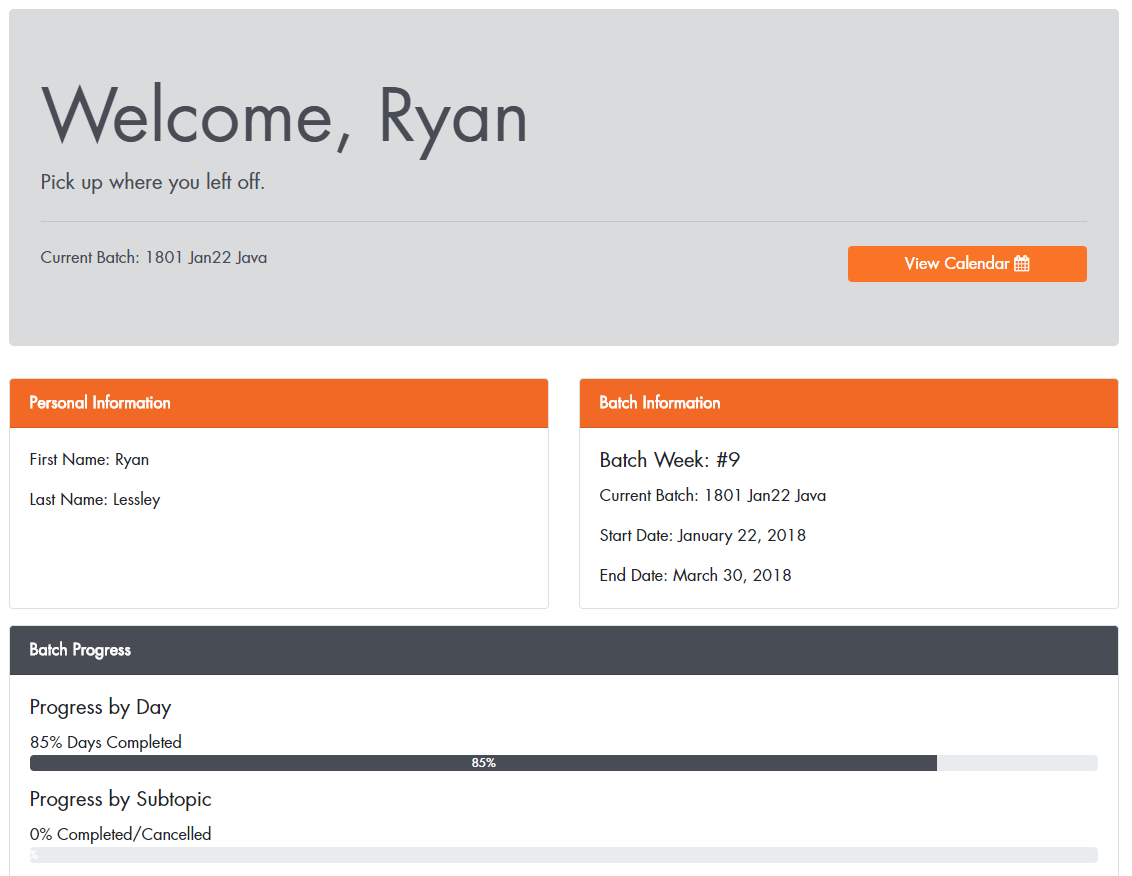
\includegraphics[width=10cm]{images/dashboard}
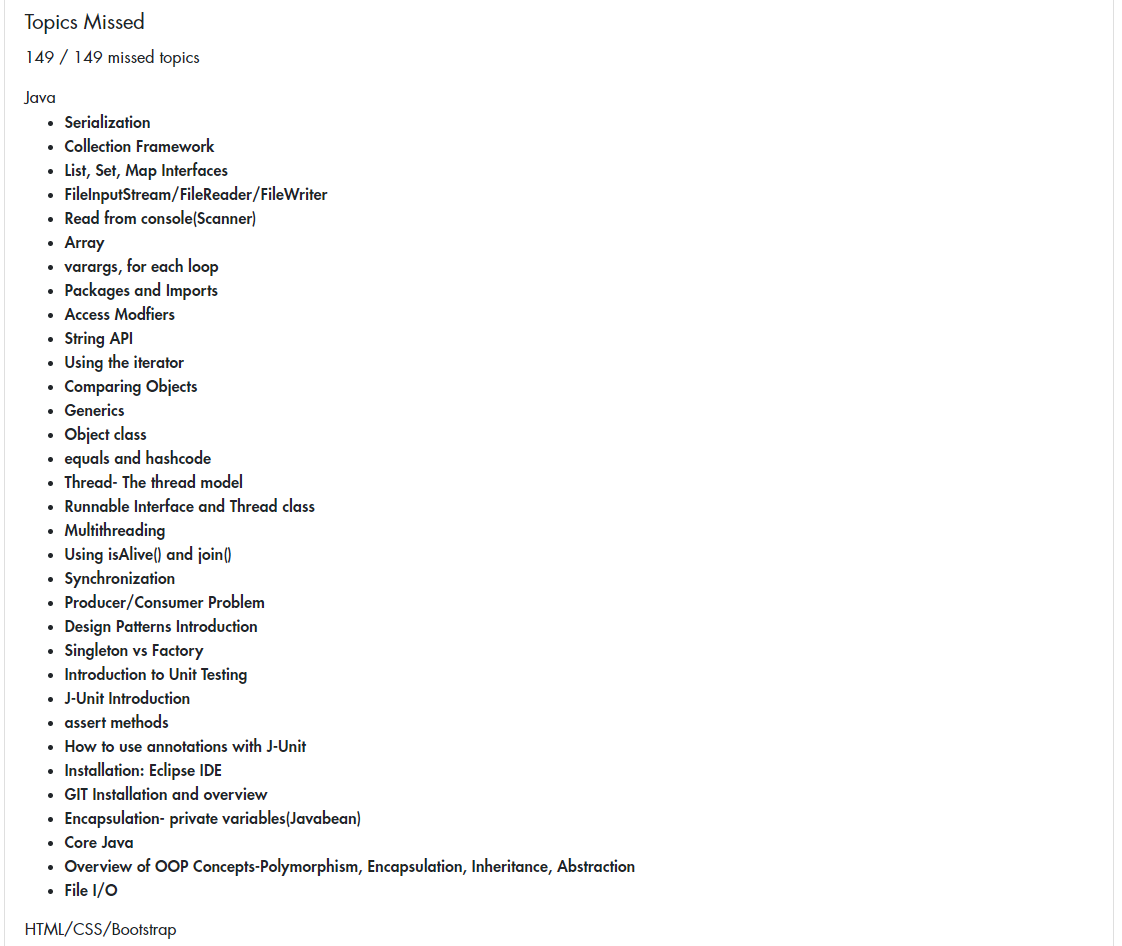
\includegraphics[width=10cm]{images/topicdash}
\caption{Bam dashboard}
\label{fig:lion}
\end{figure}
\subsection{Top section dashboard}
The top of the dashboard gives the user access to the following information:
\begin{itemize}
    \item A link to the calendar of the trainer’s current batch.
    \item Personal information about the trainer.
    \item Information about the batch.
    \item The progress of the batch, measured in number of days completed and number of subtopics completed
\end{itemize}
\subsection{Bottom section dashboard}
The bottom of the dashboard gives the user access to the following information:
\begin{itemize}
    \item A link to the calendar of the trainer’s current batch.
\end{itemize}

\begin{figure}[htp]
\centering
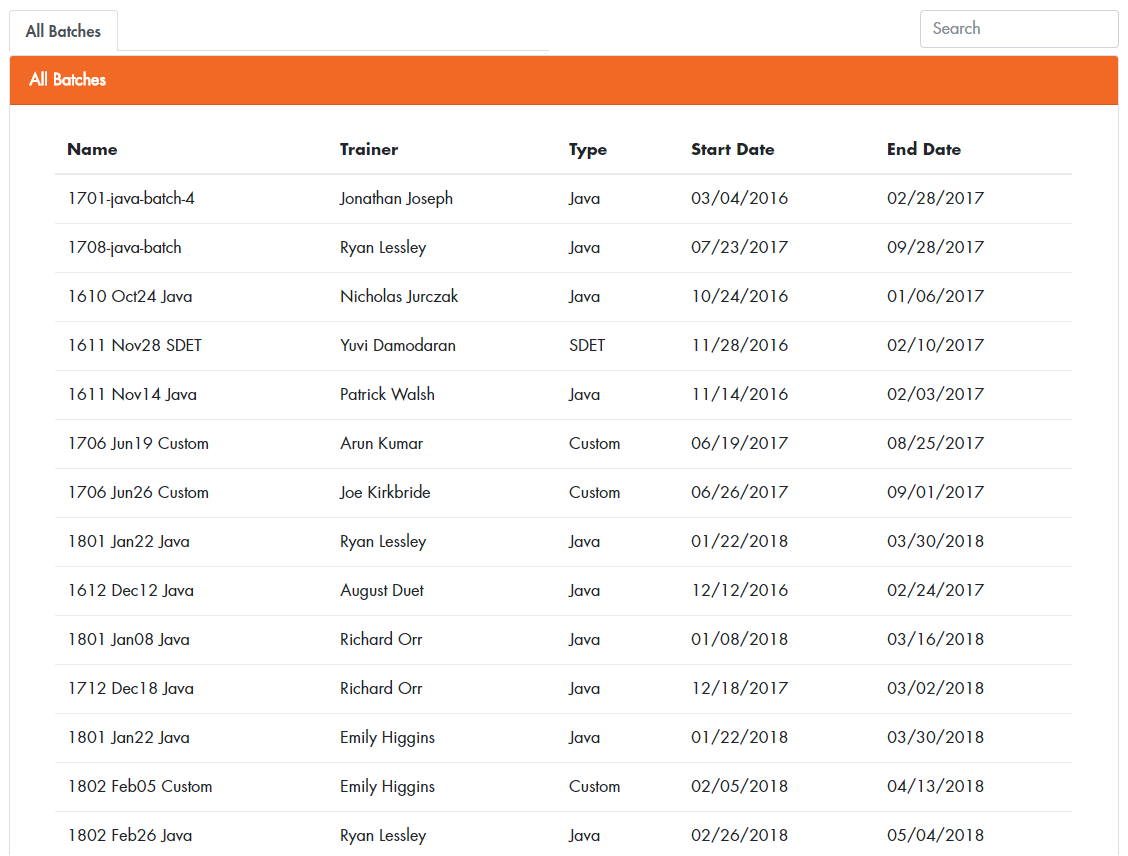
\includegraphics[width=10cm]{images/Batchview}
\caption{All Batches}
\label{fig:lion}
\end{figure}

\subsection{All Batches}
The All Batches tab gives the user access to the following functionality:

\begin{itemize}
    \item Search for keywords matching fields in the all batches table using the search bar in the top right corner.
    \item View information about all batches, including batch name, trainer, batch type, and the start and end date of the batch
\end{itemize}

\subsection{My Batch}
The My Batches tab gives the user access to the following information:

\begin{figure}[htp]
\centering
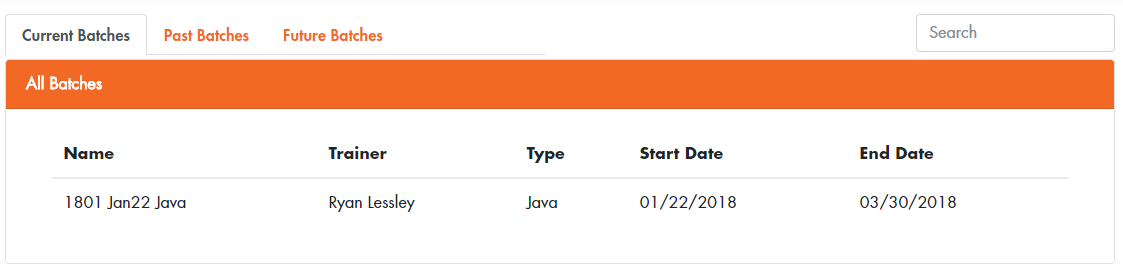
\includegraphics[width=10cm]{images/myBatch}
\caption{All Batches}
\label{fig:lion}
\end{figure}

\begin{itemize}
    \item Current Batches – Information about the batch(es) currently in progress that a trainer is responsible for
    \item Past Batches – Information about the batch(es) that have been completed that a trainer was responsible for
    \item Future Batches – Information about the batches that the trainer will be responsible for in the future
\end{itemize}

\subsection{Calender}
The Calendar grants the user the following functionality:
\begin{figure}[htp]
\centering
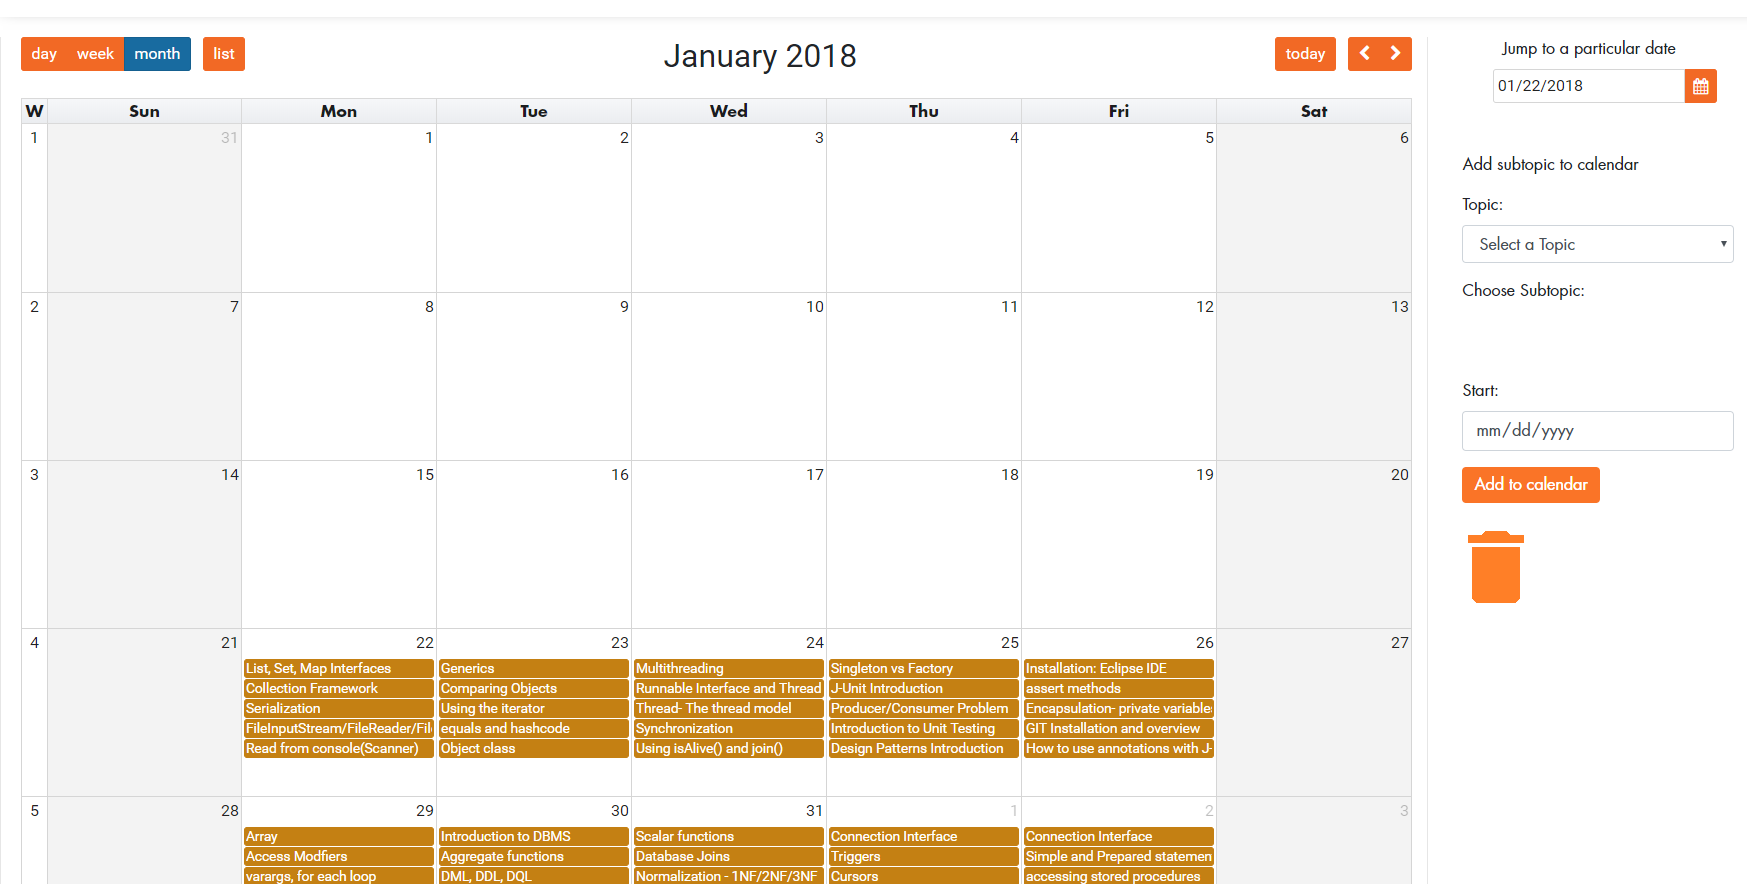
\includegraphics[width=10cm]{images/calendarView}
\caption{Calender view}
\label{fig:lion}
\end{figure}

\begin{itemize}
    \item View the schedule of subtopics to be covered on a certain date for a batch
    \item Add a subtopic to the calendar by:
    \begin{itemize}
        \item Selecting the topic the subtopic you wish to add is located.
        \item Choose the subtopic to add to the date.
        \item Select the date to cover that subtopic.
        \item Select “Add to Calendar”.
    \end{itemize}
        
    \item Add a subtopic to the calendar by:
    \begin{itemize}
        \item Selecting the topic the subtopic you wish to add is located.
        \item Dragging the subtopic to wish to add to the date on the calendar.
    \end{itemize}
        
    \item Change the status of a subtopic by:
    \begin{itemize}
        \item Clicking on the subtopic you wish to change the status of in the calendar until the status you wish to give it is reached.
    \end{itemize}
    \item Change the date a subtopic is covered by:
    \begin{itemize}
        \item Dragging the subtopic to the new date you wish to cover the subtopic.
    \end{itemize}
    \item Remove a subtopic from the schedule by:
    \begin{itemize}
        \item Dragging the subtopic you wish to remove from the schedule to the trash can icon.
    \end{itemize}
\end{itemize}
\subsection{Curriculum Editor}
The Curriculum Editor gives the user the following functionality:
\begin{figure}[htp]
\centering
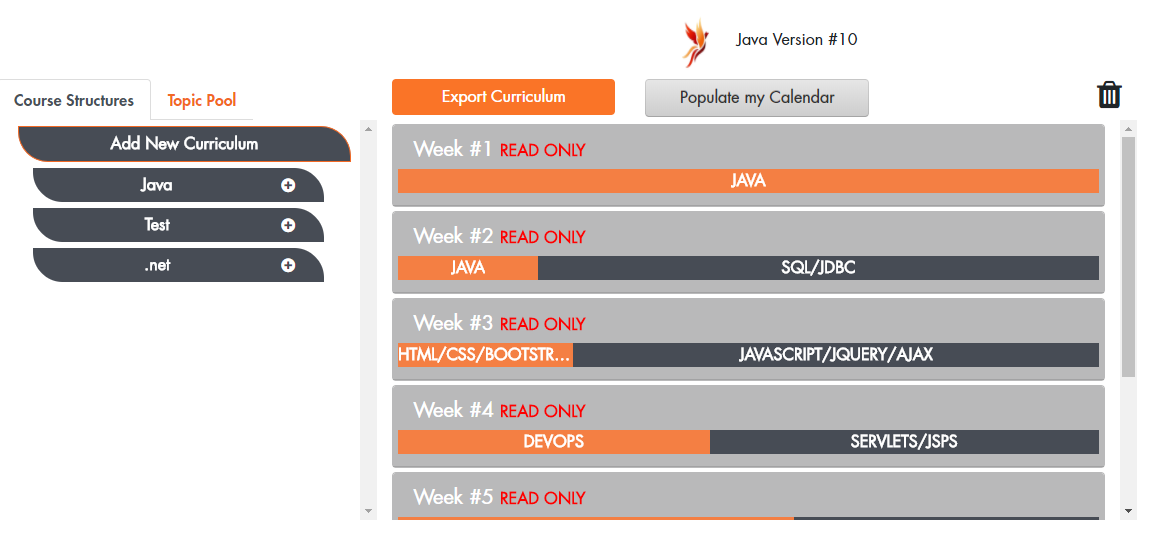
\includegraphics[width=10cm]{images/curriculumView}
\caption{Curriculum Editor}
\label{fig:lion}
\end{figure}

\begin{itemize}
    \item Export Curriculum – Exports an Excel file containing the curriculum plan based on the current curriculum in the editor
    \item Populate my Calendar – Populates the calendar for the current batch with the current curriculum in the editor
    \item Delete Curriculum Version – Delete the curriculum version by:
    \begin{itemize}
        \item Clicking the trash can icon to the top right of the Curriculum Editor when the version you wish to delete is displayed.
        \item Confirm that you want to delete that version of the curriculum.
    \end{itemize}
\end{itemize}
The Course Structures tab side menu gives the user the following functionality:
\begin{itemize}
    \item Add New Curriculum Label – Allows the user to create a new curriculum label that can maintain one or more curriculum versions by:
    \begin{itemize}
        \item Clicking “Add New Curriculum”.
        \item Entering the name of the label into the text box.
    \end{itemize}
    \item Add New Curriculum – Allows the user to create a new version of a curriculum under an existing label by:
    \begin{itemize}
        \item Clicking the “plus” symbol next to the label you wish to create a new curriculum version for.
        \item Populating each week inside of the newly created curriculum version template.
    \end{itemize}
\end{itemize}

\subsubsection{Topic Pool}
The Topic Pool tab side menu gives the user the following functionality:

\begin{figure}[htp]
\centering
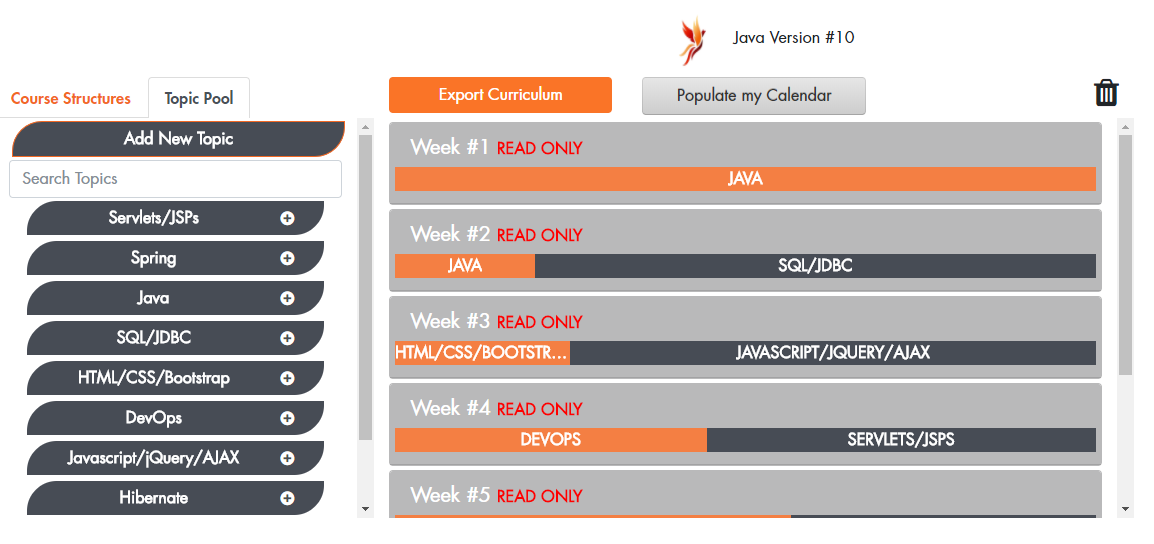
\includegraphics[width=10cm]{images/TopicView}
\caption{Topic Pool}
\label{fig:lion}
\end{figure}

\begin{itemize}
    \item Add New Topic – The user can create a new topic for the topic pool by:
    \begin{itemize}
        \item Clicking “Add New Topic”.
        \item Entering the name of the new topic into the text box.
    \end{itemize}
    \item Add New Subtopic – The user can create a new subtopic for a topic by:
    \begin{itemize}
        \item Clicking the “plus” icon next to the topic you wish to add a new subtopic to.
        \item Entering the name of the new subtopic into the text box.
    \end{itemize}
    \item Search Topics – Allows you to search for subtopics by name.
\end{itemize}
\subsection{Objectives Manager}
The Objectives Manager’s Subtopics Completion Chart gives the user the following information:

\begin{figure}[htp]
\centering
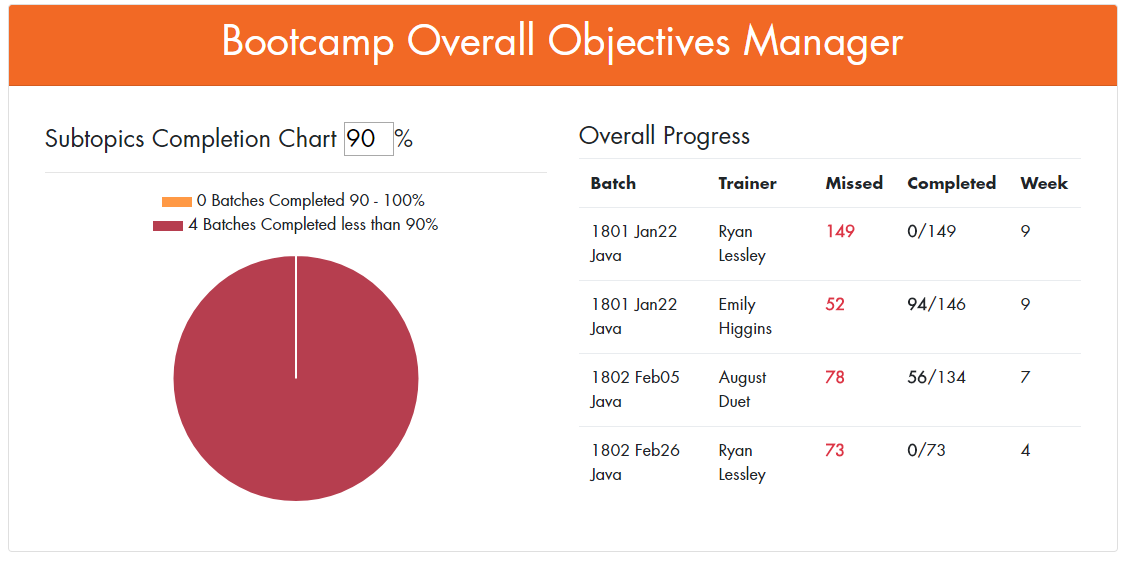
\includegraphics[width=10cm]{images/Objective}
\caption{Objectives Manager}
\label{fig:lion}
\end{figure}


\begin{itemize}
    \item A pie chart showing the number of batches that completed less than x percent of subtopics and the number of batches that completed x percent or more subtopics.
    \item An overall progress table for each active batch, showing the batch name, the trainer, number of missed and completed sub tasks, and the current week the batch is in
\end{itemize}

\begin{figure}[htp]
\centering
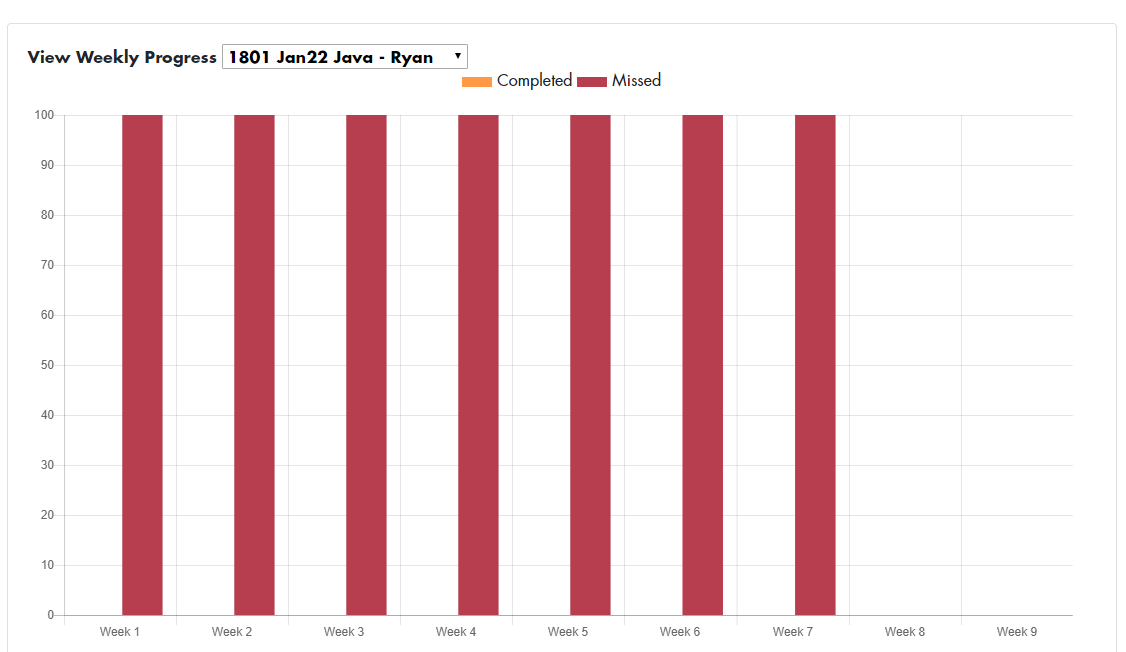
\includegraphics[width=10cm]{images/WeeklyObj}
\caption{Weekly Progress}
\label{fig:lion}
\end{figure}

The Objectives Manager’s Weekly Progress Chart gives the user the following information:
\begin{itemize}
    \item A bar graph showing the percentage of subtopics completed for each week of a batch.
\end{itemize}
